% ---------------------------------------------------------------------
% HEADER
% Formålet med å legge header til et eget dokument er å garantere at
% oppsettet av dokumentene er likt for alle løsningsforslagene.
% I headeren skjer følgende:
% (1) Dokumentet blir startet
% (2) Pakker blir importert
% ---------------------------------------------------------------------
% ---------------------------------------------------------------------
% HEADER
% Formålet med header er å importere de samme pakkene i alle dokumentene.
% ---------------------------------------------------------------------

% Sett opp dokumentet. Her kan 'twoside' brukes for printing
\documentclass[12pt, a4paper]{article}

% Vi trenger utf-8 for å bruke norske bokstaver: Æ, Ø, Å
\usepackage[utf8]{inputenc}

% Vi setter babel til norsk, da får dokumentegenskaper norske titler
\usepackage[norsk]{babel}

% For å kunne bruke grafikk
\usepackage{graphicx}
\newcommand{\figwidth}{0.75}

% Matematikkpakker fra AMS - American Mathematical Society
\usepackage{amsmath, amsthm, amsfonts, amssymb, mathtools}

% For eventuelle linker, e.g. \href{URL}{text}
\usepackage{hyperref}

% For headers og footers med eventuell logo
\usepackage{fancyhdr}

% Sett marginer manuelt
\usepackage[top = 3cm, left = 3cm, right = 3cm, bottom = 3cm]{geometry}

% For enkle lister, nyttig for oppgave a), b), c), ...
\usepackage[sharp]{easylist}

% Dersom flere kolonner er ønskelig i deler av dokumentet
\usepackage{multicol}

% For luft mellom paragrafer
\usepackage{parskip}

% For logikk assosiert med logoer
\usepackage{ifthen}

% For å finne totalt antall sider
\usepackage{lastpage}

% Annet
\usepackage{enumitem}

\usepackage{polynom}% Polynomer
\polyset{style=C, div=:}

\usepackage{systeme}% Likningssystemer

% Kan brukes når noe stryker ut noe, f.eks 1/n * n, her kan man ta \frac{1}{\cancel{n}} * \cancel{n}
\usepackage{cancel}



% ---------------------------------------------------------------------
% DOKUMENTVARIABLER
% ---------------------------------------------------------------------
\newcommand{\fagkode}{S1}
\newcommand{\semesteraar}{våren 2018}
\newcommand{\forfatter}{Tommy O.}
\newcommand{\dokumenttittel}{Løsningsforslag -- Eksamen \fagkode, \semesteraar}


% Set til 'true' og oppgi logo dersom du vil bruke en logo
\newboolean{bruklogo}
\setboolean{bruklogo}{false}
\newcommand{\logonavn}{}

% ---------------------------------------------------------------------
% SETUP
% Formålet med å legge setup til et eget dokument å garantere at headers,
% footers, og øverste del av dokumentet er likt for alle
% løsningsforslagene.
% ---------------------------------------------------------------------
% ---------------------------------------------------------------------
% HEADER
% Formålet med setup er at dokumentene ser rimelig like ut.
% ---------------------------------------------------------------------


% ---------------------------------------------------------------------
% Alternativ font. Kommentert ut fordi Computer Modern (default) er pen
%\usepackage{kmath,kerkis}
%\usepackage[T1]{fontenc}
% ---------------------------------------------------------------------


% ---------------------------------------------------------------------
% Sett opp headers og footers
\ifthenelse{\boolean{bruklogo}}{
% Dersom logo skal brukes, sett logoen oppe til høyre med bredde 4 cm
	\rhead{\includegraphics[width=3.5cm]{\logonavn}}
}{
% Dersom logo ikke skal brukes, sett tom header
	\rhead{}
} 
\rfoot{\thepage}
\cfoot{}
\lhead{}
\lfoot{{\scriptsize Forbedringsforslag? Bidra på \url{https://github.com/tommyod/matte_eksamener_VGS}.}}
\renewcommand{\headrulewidth}{0pt}
% ---------------------------------------------------------------------


% ---------------------------------------------------------------------
% To streker under svaret
\def\answer#1{\underline{\underline{#1}}}
% ---------------------------------------------------------------------


% ---------------------------------------------------------------------
% Start selve dokumentet
% ---------------------------------------------------------------------

\begin{document}
\pagestyle{fancy}
{\bfseries \Large \dokumenttittel} \\
{ \footnotesize Laget av \forfatter 
	\hfill Sist oppdatert: \today 
	\hfill Antall sider: \pageref*{LastPage}}
\hrule
\vspace{1em}
\begin{center}
\fbox{\fbox{\parbox{.90\textwidth}{
	Dette dokumentet er open-source;
	alle kan bidra til å gjøre det bedre.
	Dersom du finner skrivefeil, matematiske feil, eller ser at forklaringene kan være bedre: ikke nøl med å sende inn en endring. 
	Du kan finne siste versjon, og bidra, på GitHub, se:
	\url{https://github.com/tommyod/matte_eksamener_VGS}
}}}
\end{center}


% ---------------------------------------------------------------------
% DOKUMENTSTART - Skriv løsningsforslaget nedenfor
% ---------------------------------------------------------------------	
\section*{Del 1 - uten hjelpemidler}
\subsection*{Oppgave 1}
\begin{easylist}[enumerate]
\ListProperties(Style2*=,Numbers=a,Numbers1=l,FinalMark={)})
# Vi flytter alt over på én side av likningen, slik at vi får en andregradslikning som vi kan faktorisere med ABC-formelen (eller en annen metode).
\begin{align*}
	2x^2 - 5x + 1 &= x - 3 \\
	2x^2 - 6x + 4 &= 0 \qquad \text{(flytter over)}\\
	2 \left( x^2 - 3x + 2 \right) &= 0 \qquad \text{(trekker ut 2)} \\
	2 (x-1)(x-2) &= 0 \qquad \text{(faktoriserer)}\\
	\answer{x = 1 \text{ eller } x = 2} &	
\end{align*}

# Her flytter vi over slik at vi får logaritmen på en side alene, og deretter tar vi 10 opphøyd i begge sider av likningen for å bli kvitt logaritmen.
\begin{align*}
	2 \lg \left(x + 7\right) &= 4 \\
	\lg \left(x + 7\right) &= 2  \qquad \text{(deler på 2)}\\
	10^{\lg \left(x + 7\right)} &= 10^2  \qquad \text{(opphøyer i 10)}\\
	x + 7 &= 100 \qquad \text{(bruker at } 10^{\lg a} = a \text{ )} \\
	\answer{x = 93}
\end{align*}
# Vi samler først sammen så mye som mulig med samme grunntall, og så bruker vi egenskapen at dersom $a^x = a^y$, så må $x=y$.
\begin{align*}
	3 \cdot 2^{3x+ 2} &= 12 \cdot 2^6 \\
	3 \cdot 2^{3x+ 2} &= 3 \cdot 2 \cdot 2 \cdot 2^6 \qquad \text{(faktoriserer 12)} \\
	3 \cdot 2^{3x+ 2} &= 3 \cdot 2^8 \qquad \text{(bruker } a^n \cdot a^m = a^{n+m} \text{ )} \\
	 2^{3x+ 2} &= 2^8 \qquad \text{(deler på 3)} \\
	  {3x+ 2} &= 8 \qquad \text{(bruker } 2^x = 2^y \Leftrightarrow x = y \text{ )} \\
	  \answer{x = 2}
\end{align*}
\end{easylist}

\subsection*{Oppgave 2}
Vi skal løse likningssystemet
\begin{align*}
	(1) \quad & x^2 + 3y = 7 \\	
	(2) \quad & 3x - y = 1.
\end{align*}
Det er mange fremgangsmåter som vil fungere, og dersom man gjør det riktig så skal man få samme svar uansett. Vi velger her å først løse likning $(2)$ for $y$, og får da $y = 3x - 1$.
Dette setter vi inn i likning $(1)$:
\begin{align*}
	x^2 + 3 \left( 3x - 1\right) &= 7 \\
	x^2 + 9x - 3 &= 7 \\
	x^2 + 9x - 10 &= 0 \\
	(x + 10)(x - 1) &= 0 \\
	x = -10 \text{ eller } x = 1.
\end{align*}
Vi bruker $x$-verdiene til å finne $y$-verdier, ved å bruke likningen $y = 3x - 1$. Vi får:
\begin{align*}
	x = -10 \quad & \Rightarrow \quad y = 3(-10) - 1 = -31 \\
	x = 1 \quad \ \quad & \Rightarrow \quad y = 3(1) - 1 = 2
\end{align*}
Løsningene er altså \answer{$(x, y) = (-10, -31)$} og \answer{$(x, y) = (1, 2)$}. Som en kommentar nevnes det at dersom man plotter likningene som kurver i et koordinatsystem, vil løsningene være skjæringspunktene mellom kurvene. 
Figuren nedenfor viser dette.

\begin{center}
	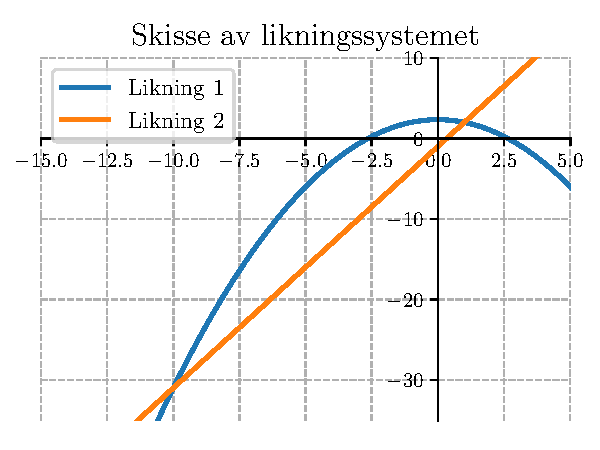
\includegraphics[width=0.55\linewidth]{figs/del1_oppg2}
\end{center}

\subsection*{Oppgave 3}
\begin{easylist}[enumerate]
	\ListProperties(Style2*=,Numbers=a,Numbers1=l,FinalMark={)})
	# Her ganger vi bare ut og kansellerer.
	Det kan være lurt å bruke andre kvadratsetning $(a-b)^2 = a^2 -2ab + b^2$ på den første parentesen.
	\begin{gather*}
		\left( 2x - 3\right)^2 - 2x \left(2x - 6\right) =\\
		4x^2 - 12x + 9 - \left[ 4x^2 - 12x\right] =\\
		4x^2 - 12x + 9 -  4x^2 + 12x = \answer{9}
	\end{gather*}
	# Her må vi huske logaritmesetningene, altså at $\lg (a^x) = x \lg (a)$ og at $\lg \left(a \cdot b\right) = \lg (a) + \lg (b)$.
	Vi viser to metoder, som begge gir samme svar.
	
	\textbf{Alternativ 1}
	\begin{gather*}
	\lg (2a) + \lg (4a) + \lg (8a) - \lg (16a) =\\
	\lg \left( \frac{2a \cdot 4a \cdot 8a}{16a} \right) 
	= 
	\lg \left( 4a^2 \right) =
	\lg (4) + \lg \left( a^2 \right) = \answer{2 \lg (2) + 2 \lg(a)}
	\end{gather*}
	
	\textbf{Alternativ 2}
	\begin{gather*}
		\lg (2a) + \lg (4a) + \lg (8a) - \lg (16a) =\\
		\lg (2) + \lg (a) + \lg (4) + \lg (a) + \lg (8) +\lg (a) - \left[\lg (16) + \lg (a)\right] =\\ 
		\lg (2) + \lg (a) + 2\lg (2) + \lg (a) + 3\lg (2) +\lg (a) - \left[4 \lg (2) + \lg (a)\right] =\\
		\lg (2) + \lg (a) + 2\lg (2) + \lg (a) + 3\lg (2) +\lg (a) - 4 \lg (2) - \lg (a) =\\
		\answer{2 \lg (2) + 2 \lg(a)}
	\end{gather*}
	# Vi må finne fellesnevner for å legge sammen brøkene. Fellesnevneren er $ab$, så vi ganger den første bøken med $b$ og den andre med $a$, både i teller og nevner.
	\begin{equation*}
		\frac{1}{a} + \frac{1}{b} - \frac{a - b}{ab} =
		\frac{b}{ab} + \frac{a}{ab} - \frac{a - b}{ab} =
		\frac{b + a - (a - b)}{ab} =
		\frac{2b}{ab} = \answer{\frac{2}{a}} 
	\end{equation*}
\end{easylist}

\subsection*{Oppgave 4}
Vi bruker ABC-formelen eller en annen metode for å faktorisere andregradspolynomet, og får $( x - 1)(x - 2) \geq 0$.
Polynomet bytter fortegn i $x = 1$ og i $x = 2$, fra negativt til positivt eller motsatt.
Vi kan finne ut når polynomet er positivt og negativ på tre ulike måter: (1) vi kan sjekke et punkt som $x = 1.5$, (2) lage en fortegnslinje eller (3) argumentere med at fortegnet i andregradsleddet $x^2$ er positivt---da vokser funksjonen når $x$ blir stor eller liten, og polynomet er bare negativt når $1 < x < 2$.
\begin{equation*}
	x^2 - 3x + 2 \geq 0 
	\quad \Rightarrow \quad ( x - 1)(x - 2) \geq 0
	\quad \Rightarrow \quad \answer{x \leq 1 \text{ eller } x \geq 2}.
\end{equation*}

\subsection*{Oppgave 5}
\begin{easylist}[enumerate]
	\ListProperties(Style2*=,Numbers=a,Numbers1=l,FinalMark={)})
	# I Pascals trekant er hvert tall summen av de to tallene ovenfor.
	De første åtte radene ser slik ut.
	\begin{gather*}
	1 \\
	1 \quad 1 \\
	1 \quad 2 \quad 1 \\
	\textbf{1} \quad 3 \quad 3 \quad 1 \\
	1 \quad 4 \quad 6 \quad \textbf{4} \quad 1  \\
	1 \quad 5 \quad 10 \quad 10 \quad 5 \quad 1  \\
	1 \quad 6 \quad 15 \quad 20 \quad 15 \quad 6 \quad 1 \\
	1 \quad 7 \quad 21 \quad \textbf{35} \quad 35 \quad 21 \quad 7 \quad 1 
	\end{gather*}
	Dersom man teller radene og kolonnene med å starte fra null, finner vi binomialkoeffisienten $\binom{n}{k}$ i rad $n$, kolonne $k$.
	De tallene som vi trenger i neste deloppgave er merket med fet skrift.
	
	# Det er 3 røde kuler og 4 blå. Sannsynligheten for å trekke 3 blå er antall mulige måter å trekke 3 blå og 0 røde, delt på antall mulige måter å trekke 3 kuler totalt.
	Vi henter binomialkoeffisientene fra Pascals trekant i forrige oppgave.
	\begin{equation*}
		P(3\text{ blå}) = \frac{\text{antall gunstige}}{\text{antall mulige}}
		= \frac{\binom{4}{3} \cdot \binom{3}{0}}{\binom{7}{3}} = 
		\frac{4 \cdot 1}{35} = \answer{\frac{4}{35}}
	\end{equation*}
	
	# Vi presenterer to ulike måter å løse oppgaven på. Begge gir samme svar.
	
	\textbf{Alternativ 1}
	\begin{center}
		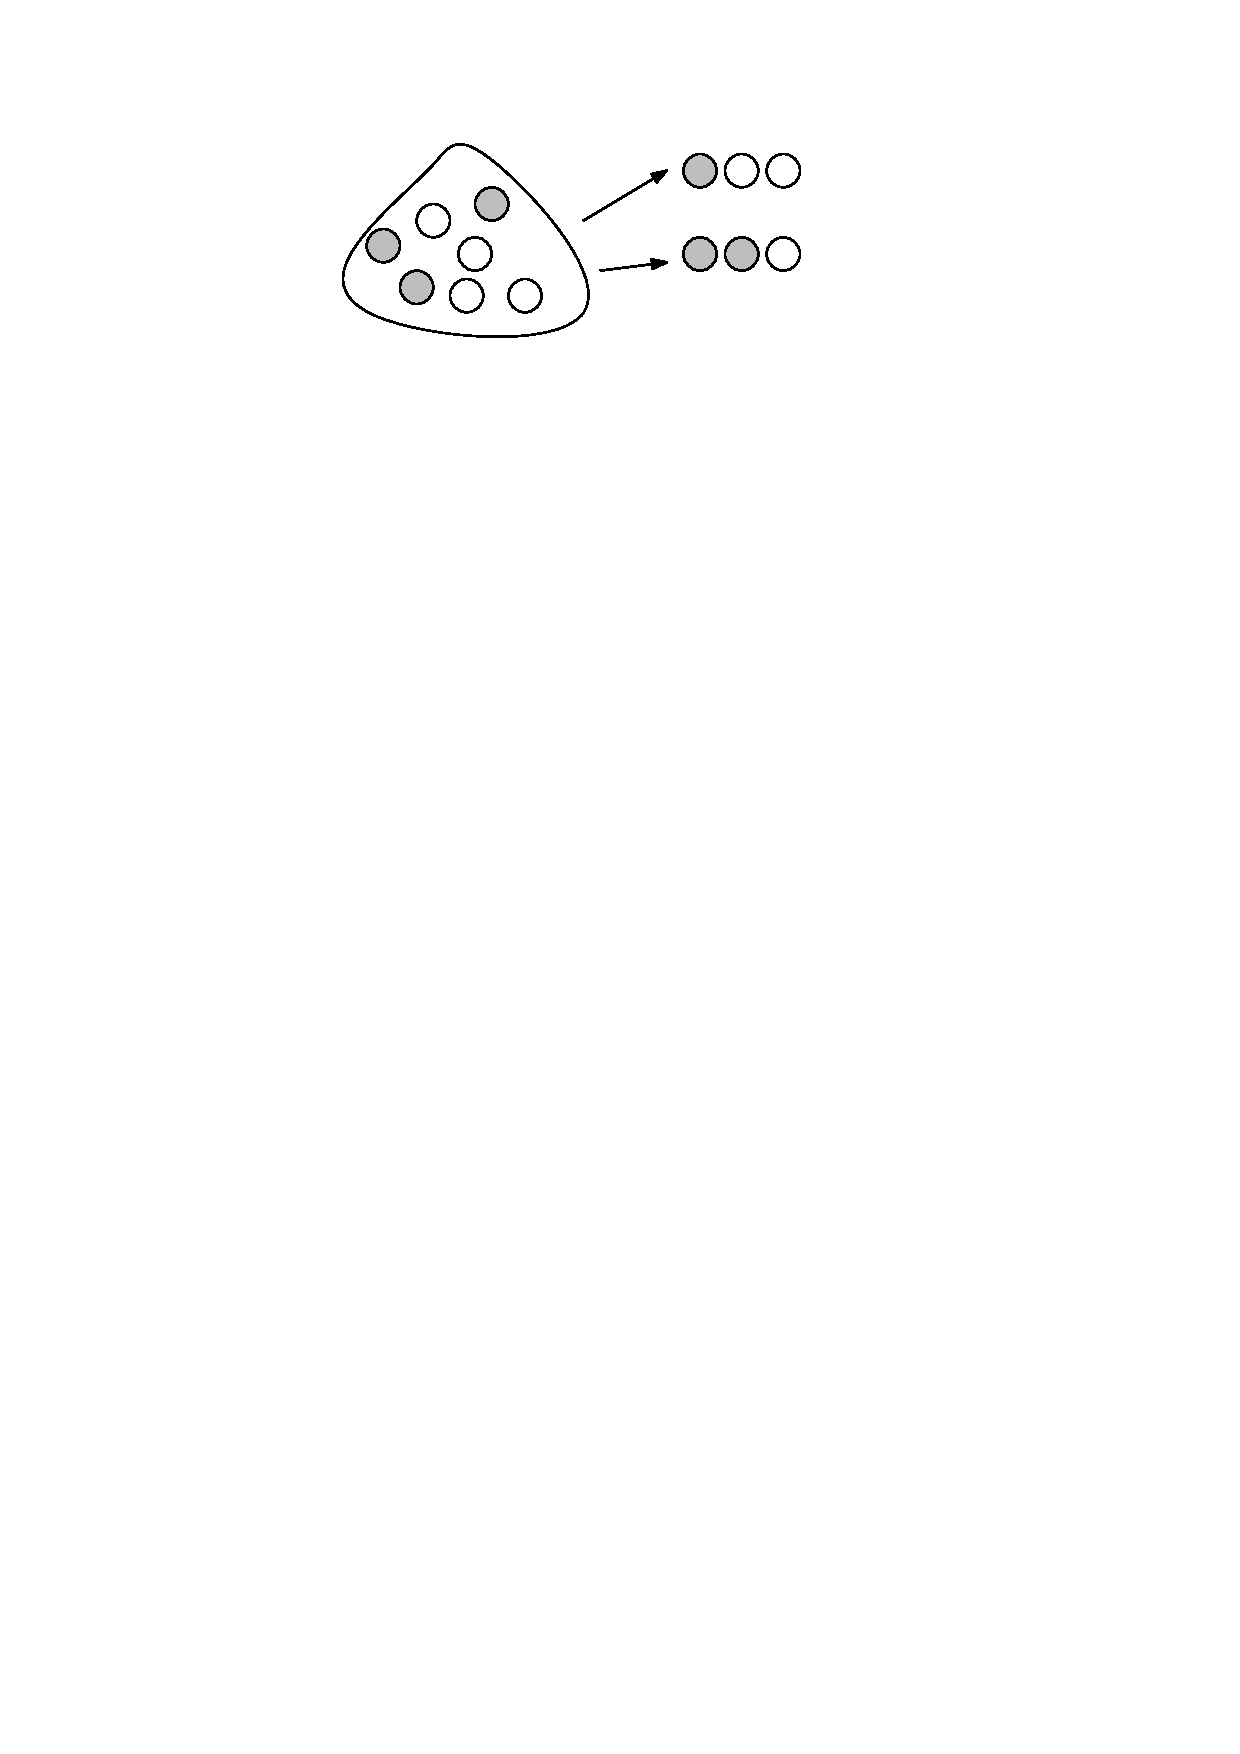
\includegraphics[width=0.4\linewidth]{figs/del1_oppg5_1}
	\end{center}
	Dersom vi skal trekke 3 kuler, og vi må minst ha én av hver farge, er det to måter å gjøre dette på: enten ved å trekke 1 rød og 2 blå, eller ved å trekke 2 røde og 1 blå. Se figuren ovenfor\footnote{Figuren er i sort/hvitt. De røde kulene er illustrert som gråe, og de blå som hvite.}. Vi kan legge sammen sannsynlighetene slik:
	\begin{equation*}
		P(\text{1 rød, 2 blå}) + P(\text{2 røde, 1 blå}) = \frac{\binom{3}{1}\binom{4}{2}}{\binom{7}{3}}
		+
		\frac{\binom{3}{2}\binom{4}{1}}{\binom{7}{3}} = \frac{3 \cdot 6 + 3 \cdot 4}{35}  = \answer{\frac{6}{7}}
	\end{equation*}
	
	\textbf{Alternativ 2}
	
	Her er en annen fremgangsmåte.
	La $R$ være antall røde, og $B$ være antall blå.
	For å finne sannsynligheten for at det er minst én blå ($B \geq 1$) og minst én rød ($R \geq 1$) kan vi dele opp hendelsesrommet som vist i figuren nedenfor, og regne ut alle sannsynlighetene. Summen av disse sannsynlighetene må være 1, og sannsynligheten som er ukjent er vist med et spørsmålstegn.
	\begin{center}
		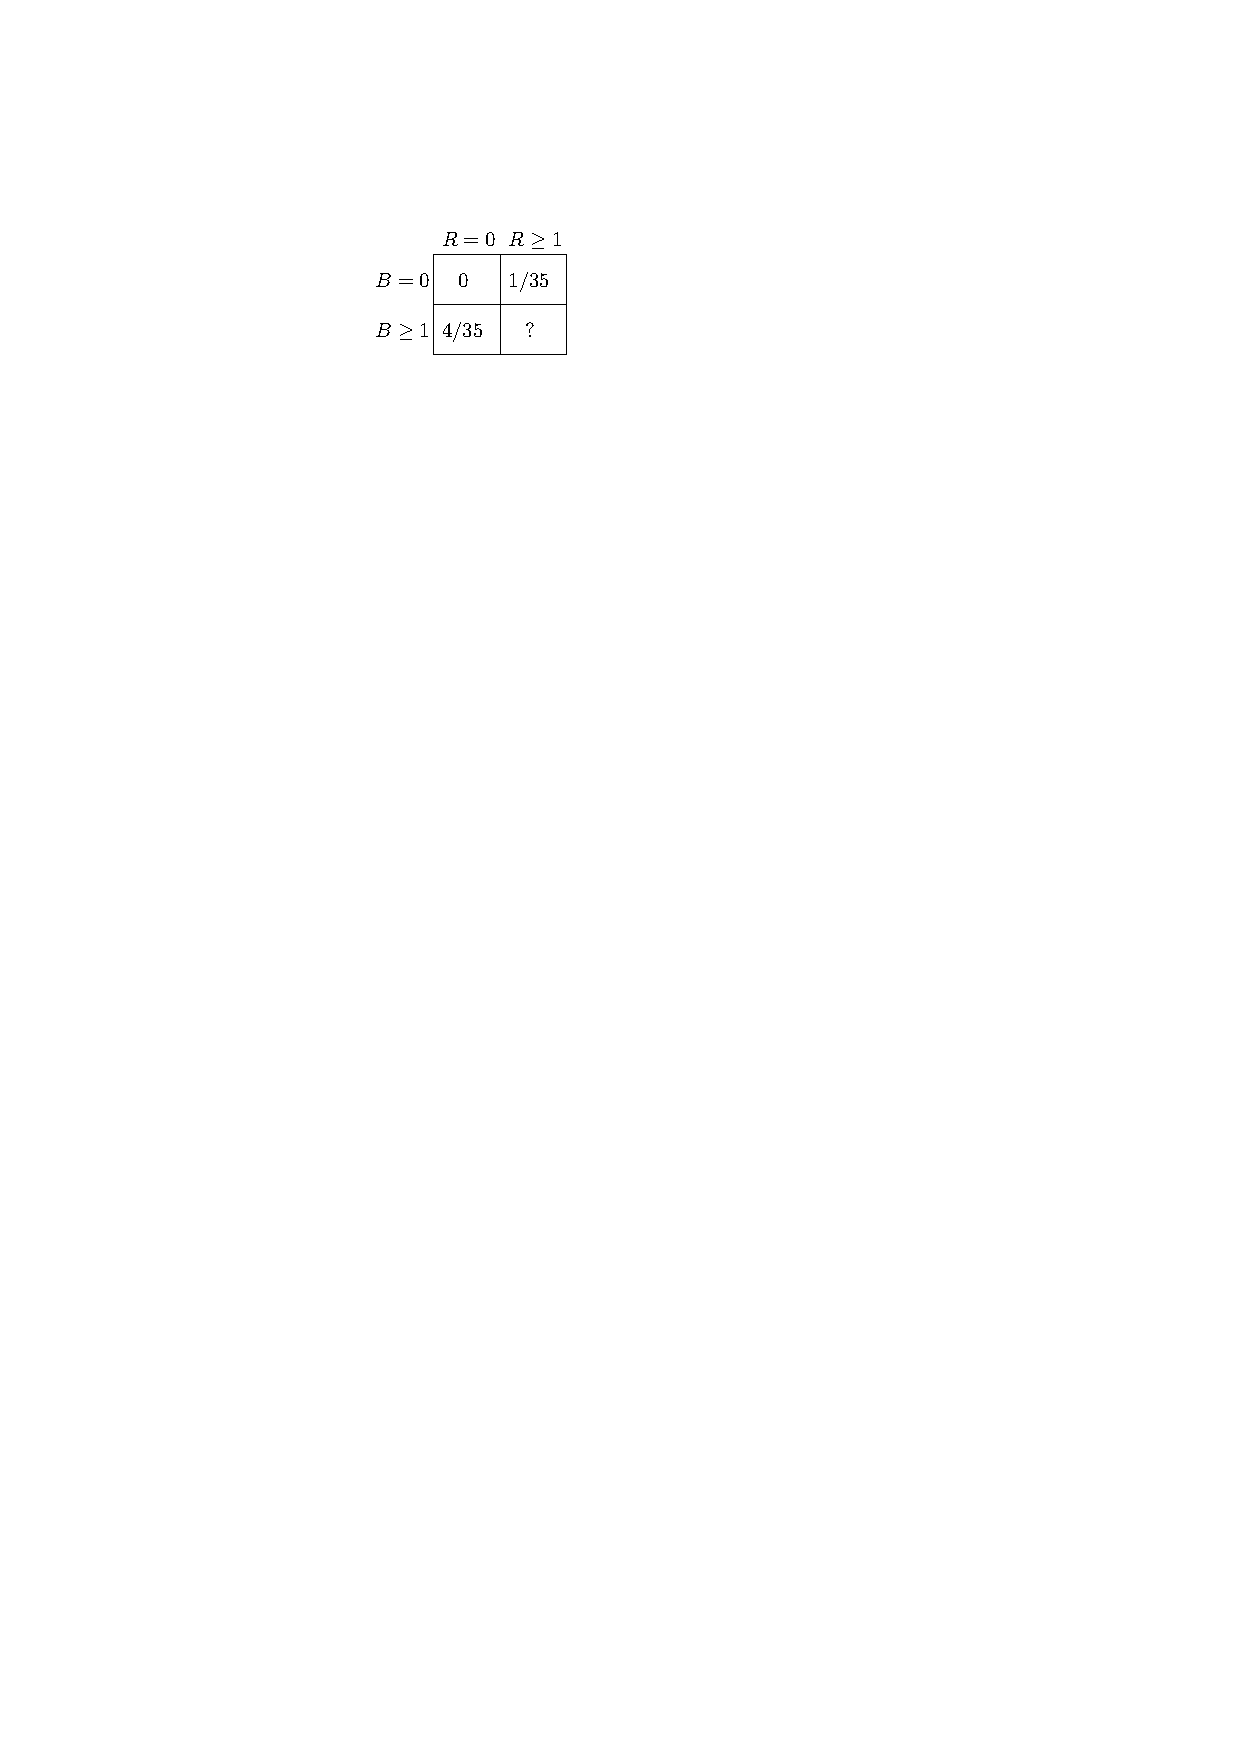
\includegraphics[width=0.25\linewidth]{figs/del1_oppg5}
	\end{center}
	Vi ser at
	\begin{align*}
		P(R = 0 \cap B = 0) &= 0  \quad \text{(umulig, fordi vi må trekke 3 kuler)}\\
		P(R \geq 1 \cap B = 0) &= \frac{1}{35} \quad \text{(kun én måte å velge ingen blå på)}\\
		P(R = 0 \cap B \geq 1) &= \frac{4}{35} \quad \text{(dette er svaret på forrige deloppgave)}
	\end{align*}
	og ettersom summen av alle sannsynligheten må være 1, kan vi regne ut at
	\begin{equation*}
		P(R \geq 1 \cap B \geq 1) = 1 -
		\left( 0 + 
		\frac{1}{35} + 
		\frac{4}{35}\right) = \frac{30}{35} = \answer{\frac{6}{7}}
	\end{equation*}
\end{easylist}

\subsection*{Oppgave 6}
Ulikhetene $x \geq 0$ og $y \leq 8$ burde være enkle å skissere.
Ulikheten $x + y \leq 10$ sier at summen må være mindre enn eller lik 10, og burde også være rimelig enkel. Den siste ulikheten kan vi skrive om til $y \geq 1 + \frac{3}{2}x$, og da er det muligens lettere tegne linja.
I figuren nedenfor er det grå området avgrenset av alle ulikhetene.

\begin{center}
	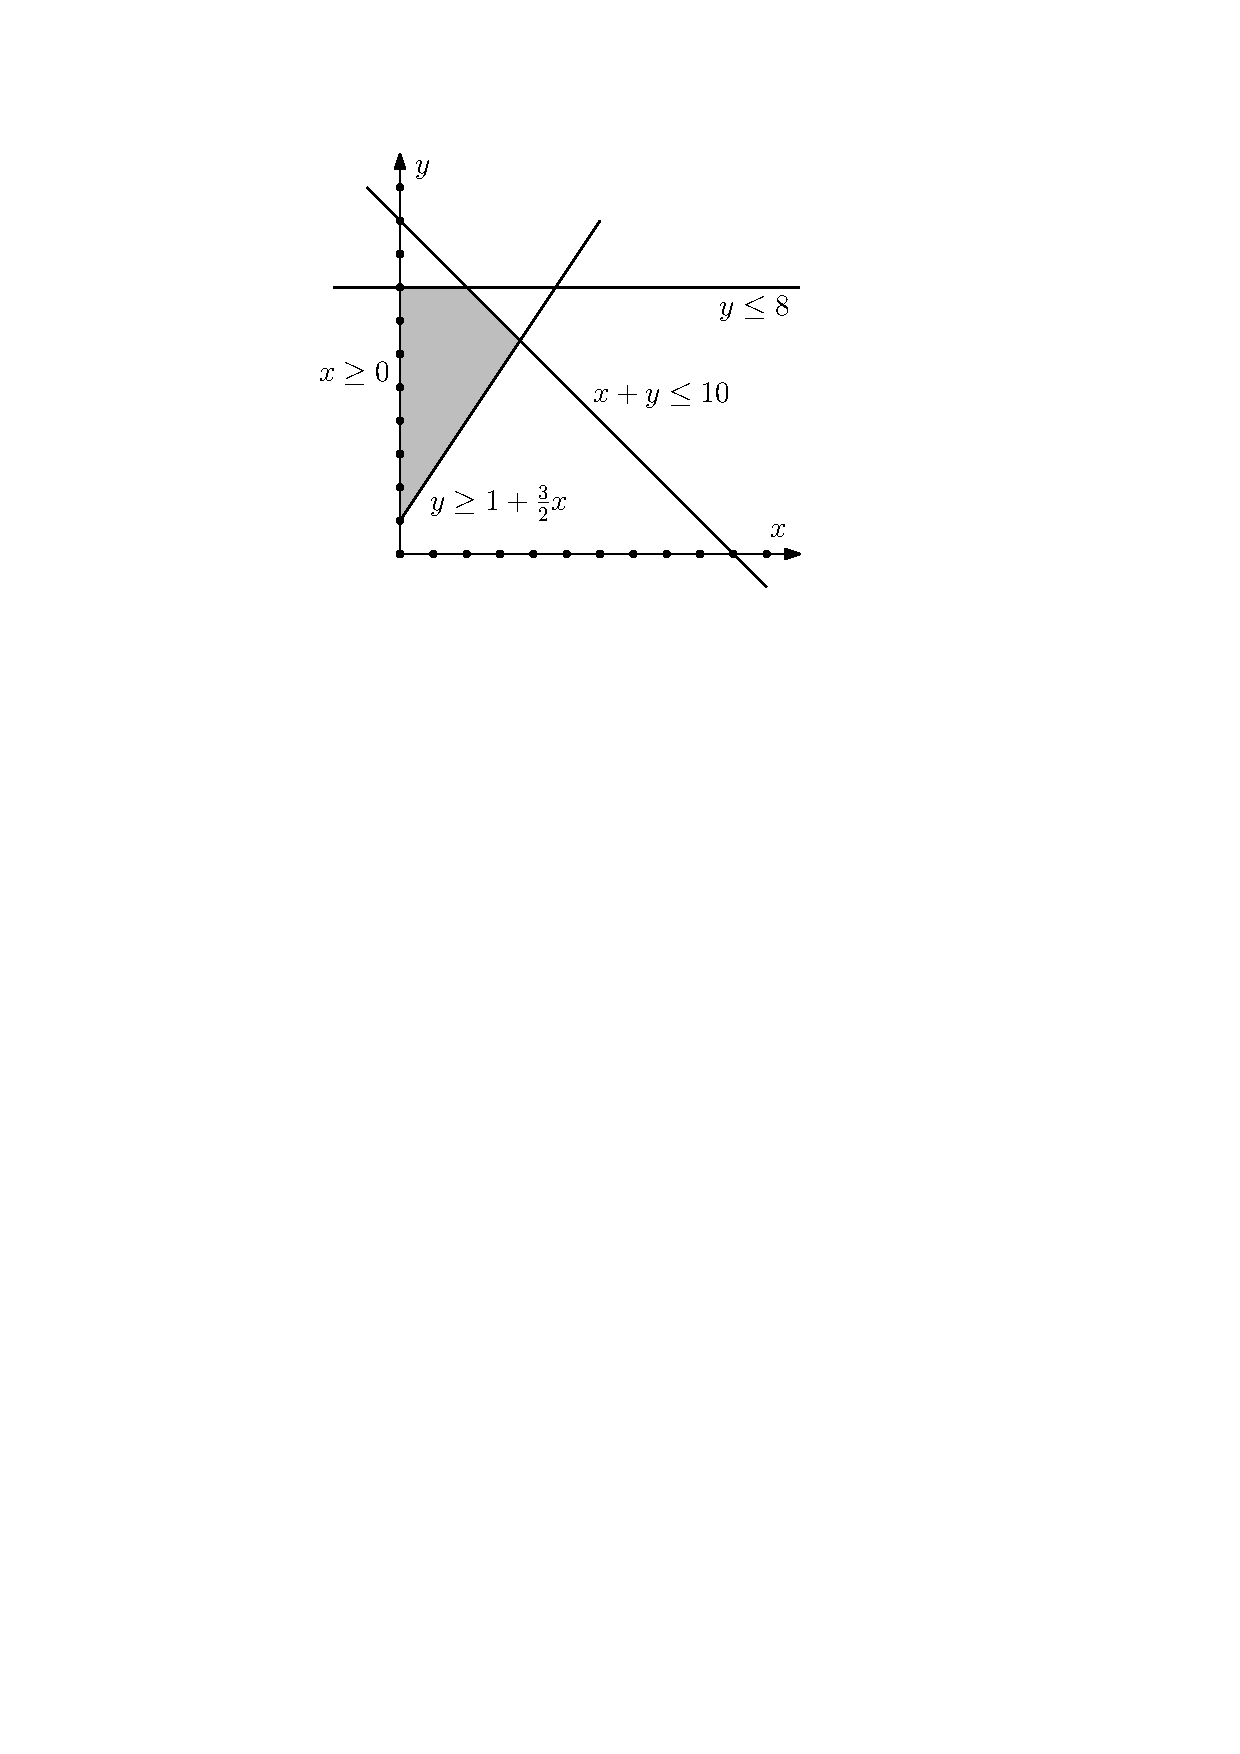
\includegraphics[width=0.5\linewidth]{figs/del1_oppg6}
\end{center}


\subsection*{Oppgave 7}
\begin{easylist}[enumerate]
	\ListProperties(Style2*=,Numbers=a,Numbers1=l,FinalMark={)})
	# Vi ser av funksjonsuttrykket at $x = -2$ er en vertikal asymptote, og at $y = 2$ er en horisontal asymptote. 
	En verikal asymptote oppstår når vi deler på null, mens en vertikal asymptote oppstår når funksjonen går mot et endelig tall når $x$ går mot positivt eller negativt evig.
	Når vi har funnet asymptotene kan vi gjøre noen stikkprøver, av f.eks. $f(0)$ og $f(-4)$, og dette gir oss nok informasjon til å skissere grafen.
	Se figuren nedenfor.
	\begin{center}
		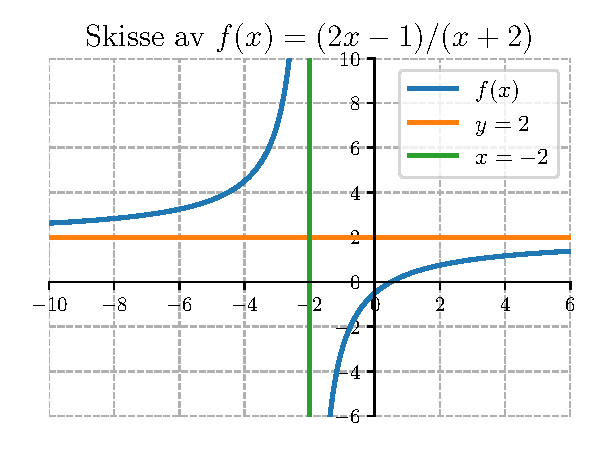
\includegraphics[width=0.55\linewidth]{figs/del1_oppg7}
	\end{center}
	
	# Vi setter $f(x)$ lik $x-2$ og løser slik:
	\begin{align*}
		\frac{2x - 1}{x + 2} = x - 2 &\quad \Rightarrow \quad 2x - 1 = (x-2)(x+2) \quad \Rightarrow \quad 2x - 1 = x^2 - 2^2 \\
		x^2 - 2x - 3 = 0  &\quad \Rightarrow \quad (x+1)(x-3) = 0 \quad \Rightarrow \quad
		\answer{x = -1 \text{ eller } x=3}
	\end{align*}
\end{easylist}

\subsection*{Oppgave 8}
\begin{easylist}[enumerate]
	\ListProperties(Style2*=,Numbers=a,Numbers1=l,FinalMark={)})
	# Her må vi bruke derivasjonsregelen $\left(x^k\right)' = k x^{k-1}$. Vi får løsningen
	\begin{equation*}
		g'(x) = 2 \cdot 3 x^{3-2} + 3 \cdot 2 x^{2-1} - 12 = \answer{6x^2 + 6x - 12}.
	\end{equation*}
	# Dersom vi har toppunkt eller bunnpunkt, må $g'(x)= 0$ i disse punktene. Vi setter $g'(x) = 0$ og løser likningen for $x$. Vi får da
	\begin{equation*}
		g'(x) = 6x^2 + 6x - 12 = 6(x^2 + x - 2) = 6(x+2)(x-1)= 0.
	\end{equation*}
	Fra dette ser vi at $g'(x) = 0$ når $x = -2$ og når $x = 1$. Vi må finne ut om dette er toppunkt eller bunnpunkt. Dette kan vi gjøre med en fortegnslinje.
	\begin{center}
		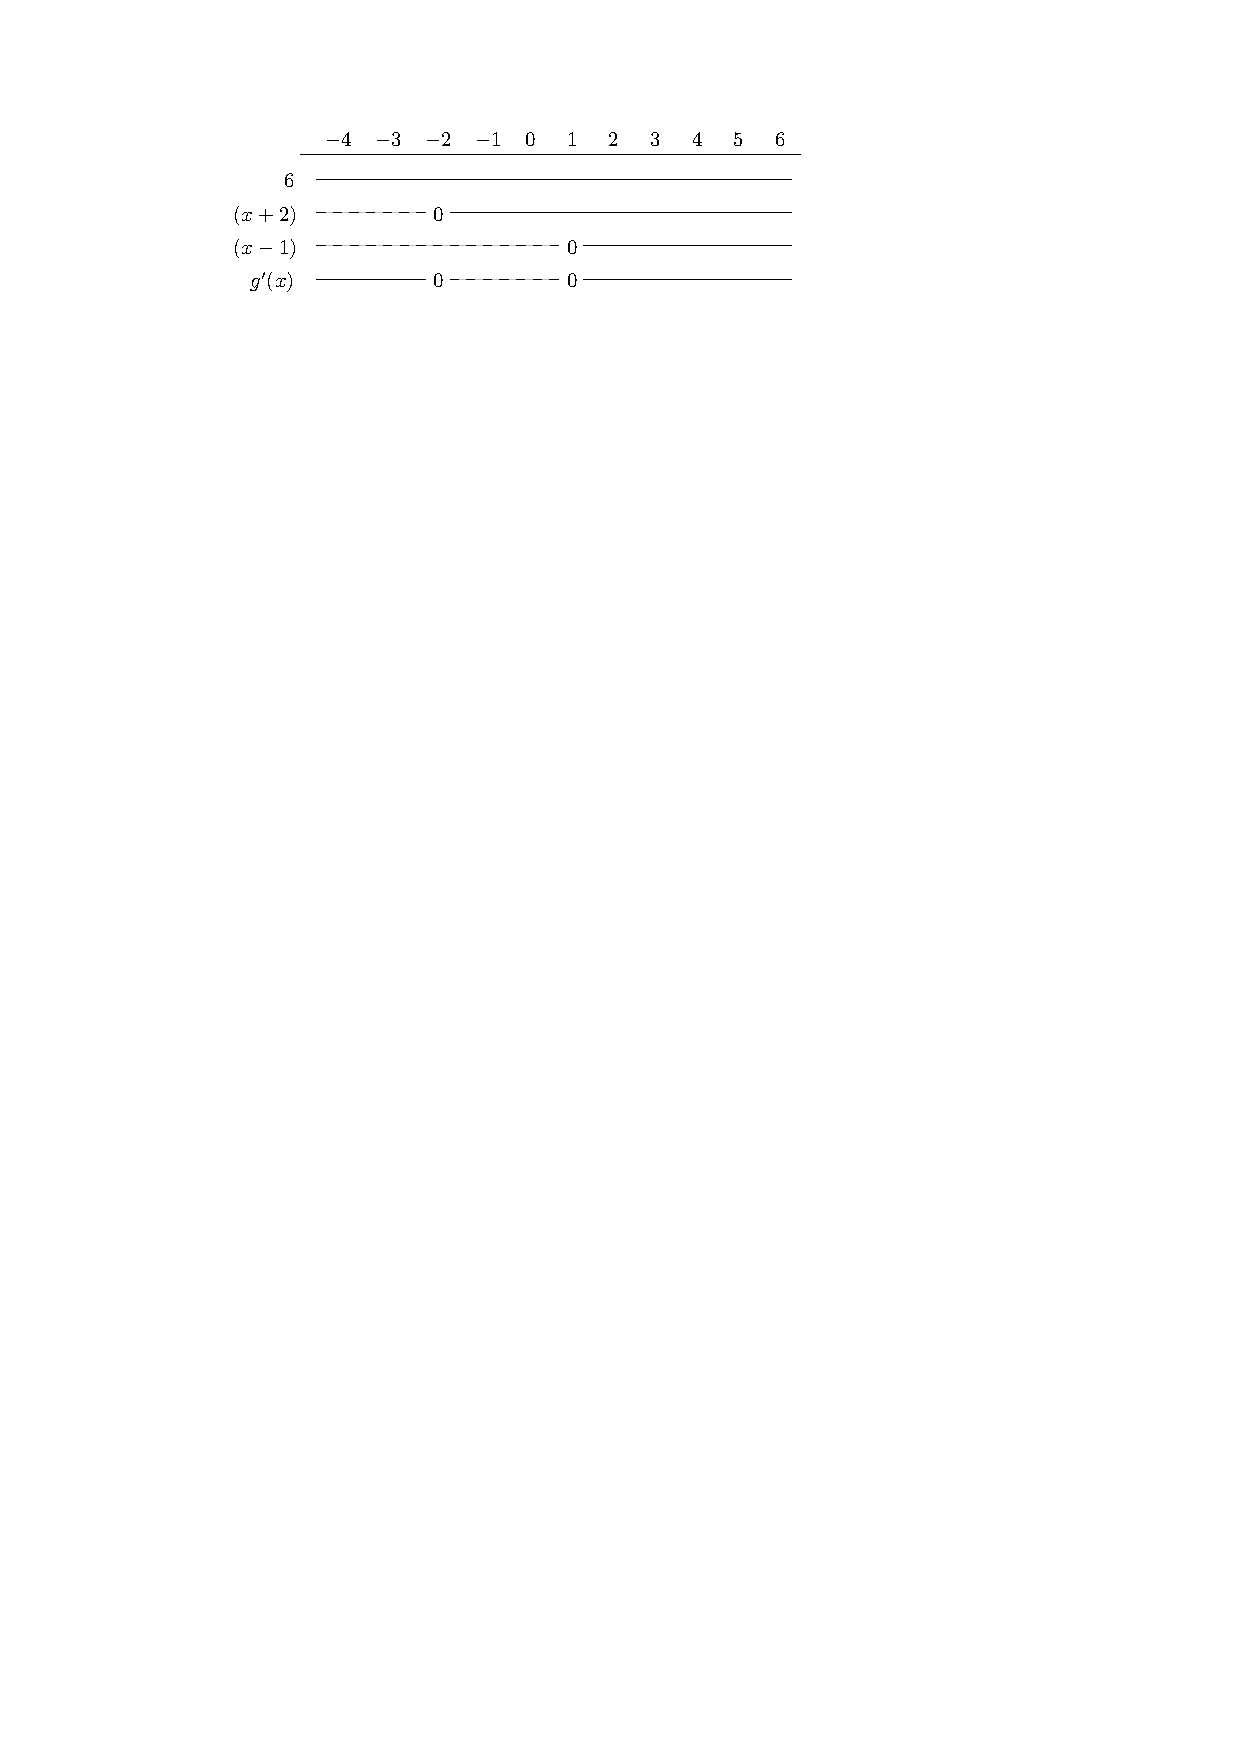
\includegraphics[width=0.8\linewidth]{figs/del1_oppg8_fortegn}
	\end{center}
	Ettersom funksjonen stiger før $x=-2$ og synker etterpå, må $x=-2$ være assosiert med et toppunkt. Tilsvarende logikk sier oss at $x=1$ er et bunnpunkt.
	\begin{align*}
		x = -2 \quad \Rightarrow& \quad y = g(-2) = 2(-2)^3 + 3 (-2)^2 - 12(-2) = -16 + 12 + 24 = 20 \\
		x = 1 \quad \Rightarrow& \quad y = g(1) = 2(1)^3 + 3 (1)^2 - 12(1) = 2 + 3 - 12 = -7
	\end{align*}
	Altså er \answer{$(-2, 20)$ et toppunkt} og \answer{$(1, -7)$ et bunnpunkt}.
	# Den gjennomsnittlige vekstfarten er endring i $y$ delt på endring i $x$, altså
	\begin{equation*}
		\frac{\Delta y}{\Delta x} = \frac{\Delta g(x)}{\Delta x} = \frac{g(2) - g(0)}{2 - 0} = \frac{g(2) - g(0)}{2 - 0} = \frac{4 - 0}{2} = \answer{2}.
	\end{equation*}
	# Den momentane vekstfarten er verdien til den deriverte.
	At den momentane vekstfaren er 24, betyr at vi må løse $g'(x) = 24$. 
	Vi løser denne likningen slik:
	\begin{align*}
		g'(x) = 6x^2 + 6x - 12 &= 24 \\
		6(x^2 + x - 6) &= 0 \\
		6(x + 3)(x - 2) &= 0.
	\end{align*}
	Vi ser at $x$-verdiene er $2$ og $-3$. Vi renger ut $y$-verdiene:
	\begin{align*}
	x = 2 \quad \Rightarrow& \quad y = g(2) = 2(2)^3 + 3 (2)^2 - 12(2) = 16 + 12 - 24 = 4\\
	x = -3 \quad \Rightarrow& \quad y = g(-3) = 2(-3)^3 + 3 (-3)^2 - 12(-3) = -54 + 27 + 36 = 9
	\end{align*}
	Den momentane vekstfaren er $24$ i punktene \answer{$(2, 4)$} og \answer{$(-3, 9)$}.
\end{easylist}

\subsection*{Oppgave 9}
\begin{easylist}[enumerate]
	\ListProperties(Style2*=,Numbers=a,Numbers1=l,FinalMark={)})
	# Grafen stiger når $f'(x) > 0$, og synker når $f'(x) < 0$.
	Vi ser fra fortegnslinjen at \answer{$f(x)$ stiger når $x < -2$ og $-2 < x <1$, og at $f(x)$ synker når $x > 1$}.
	# Her må vi skissere en funksjon som stiger, stopper å stige, stiger videre og deretter synker. 
	Den skal ha et terrassepunkt, og et toppunkt.
	Basert på fortegnslinjen kan vi anta at den deriverte er $f'(x) = (x+2)^2 (1-x)$. Både en skisse av en funksjon $f'(x)$ og dens deriverte er inkludert i figuren nedenfor.
	\begin{center}
		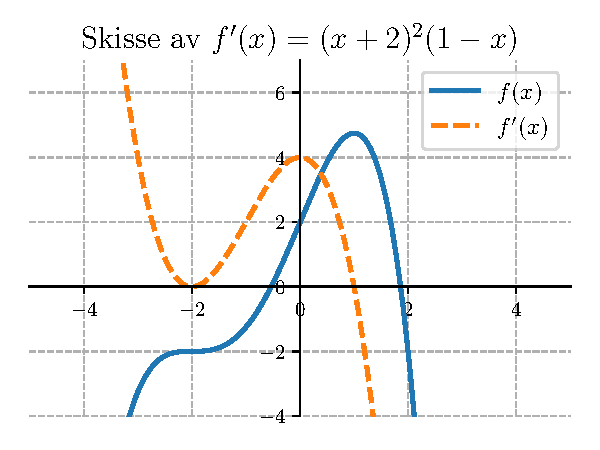
\includegraphics[width=0.55\linewidth]{figs/del1_oppg9b}
	\end{center}
\end{easylist}



\section*{Del 2 - med hjelpemidler}


\subsection*{Oppgave 1}
\begin{center}
	
\includegraphics[width=0.5\linewidth]{figs/del2_oppg1}
\end{center}
Vi lar $t$ være prisen per kilo torsk, og $s$ være prisen per kilo sei.
Basert på oppgaveteksten setter vi opp følgende likninger
\begin{align*}
	110t + 200 s &= 6795\\
	150t + 230 s &= 8390.
\end{align*}
Det er ofte en god sjekk at enhetene i likningen stemmer. I dette tilfellet er enhetene
\begin{equation*}
	\frac{\text{pris}}{\text{kilo}} \times \text{kilo} +
	\frac{\text{pris}}{\text{kilo}} \times \text{kilo} =  \text{pris},
\end{equation*}
og kansellerer man kilo på venstre siden er enhetene like.
I praksis løser vi slike oppgave i CAS i Geogebra ved å skrive \\
\verb|Løs[{110 * t + 200 * s = 6795, 150 * t + 230 * s = 8390}, {t, s}]| \\
og vi finner at \answer{$t = 24.5$ og $s = 20.5$}.

\subsection*{Oppgave 2}
\begin{easylist}[enumerate]
	\ListProperties(Style2*=,Numbers=a,Numbers1=l,FinalMark={)})
	# For å bruke en binomisk sannsynlighetsmodell må følgende forutsetninger være oppfylt\footnote{Forutsetningen om uavhengighet er nok brutt i virkeligheten, eksempelvis med familier som reiser sammen. Om foreldrene ikke møter opp, møter neppe barna heller.}:
	## Uavhengige delforsøk -- Om én enkeltperson møter opp eller ikke, påvirker ikke de andre personene.
	## Binært utfall -- Det er kun to muligheter: enten møter man opp med sannsynlighet $p$, eller ikke med sannsynlighet $1 - p$.
	## Samme sannsynlighet -- Alle har lik sannsynlighet $p$ for å møte opp.
	# Dette er binomisk forsøk med $n = 122$ og sannsynlighet $p = 0.94$, som er sannsynligheten for at en tilfeldig person møter opp. La $X$ være antall personer som møter opp totalt. Dersom flere enn 116 personer møter, får ikke alle plass. Dersom $X \leq 116$ får derimot alle plass.
	Fra sannsynlighetskalkulatoren i Geogebra finner vi at
	\begin{equation*}
		P(X \leq 116) = 0.7466 \approx \answer{74.7 \%}.
	\end{equation*}
	# La $X_n$ være antall personer som møter opp totalt, når $n$ billetter er solgt. Vi ønsker å finne den største $n$ slik at $P(X_n \leq 116) \geq 0.95$, med andre ord største antall personer vi kan selge til, slik at sannsynligheten for at alle får plass er minst 95 \%.
	Vi prøver oss frem med forskjellige $n$-verdier i Geogebra, og får
	\begin{align*}
		P(X_{116} \leq 116) &= 1 \\
		P(X_{117} \leq 116) &= 0.9993 \\
		P(X_{118} \leq 116) &= 0.9942 \\
		P(X_{119} \leq 116) &= 0.9764 \\
		P(X_{120} \leq 116) &= 0.934 
	\end{align*}
	Fra dette ser vi at største antall billetter som kan selges er \answer{$n=119$}.
	Hele sammenhengen mellom antall billetter solgt, og sannsynligheten for at alle får plass, er vist i plottet nedenfor. Dette er ikke en del av svaret, det er kun inkludert som en bonus.
	\begin{center}
		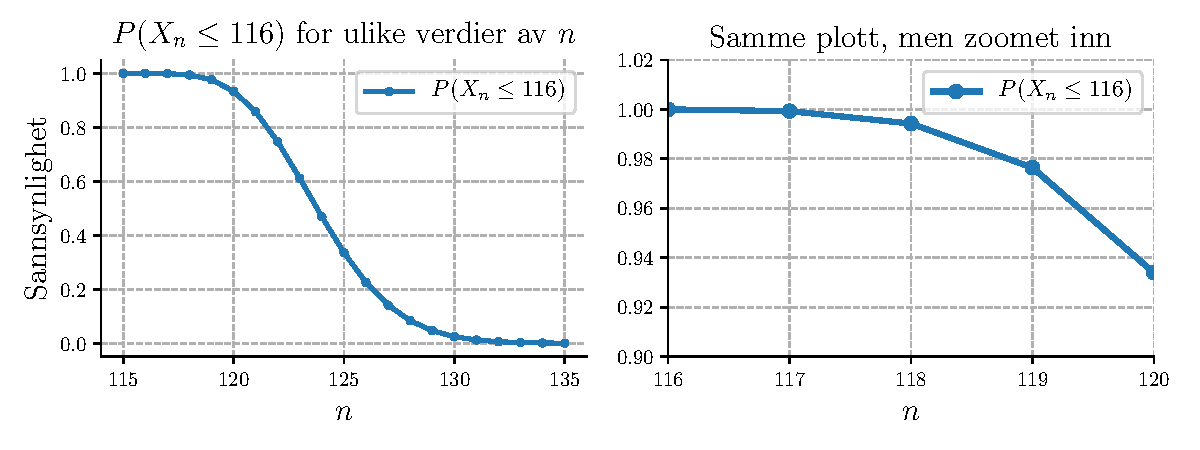
\includegraphics[width=0.99\linewidth]{figs/del2_oppg2}
	\end{center}
\end{easylist}


\subsection*{Oppgave 3}
\begin{easylist}[enumerate]
	\ListProperties(Style2*=,Numbers=a,Numbers1=l,FinalMark={)})
	# Vi bruker setningene fra oppgaven til å sette opp ulikheter. Dersom Frode bruker 10 minutter på en kasse av type A, og det blir produsert $x$ av disse, bruker han totalt $10x$ minutter på kasser av denne typen. På samme måte, dersom han bruker 30 minutter på en kasse av type B, og det blir produsert $y$ av disse, bruker han totalt $30y$ minutter på kasser av denne typen. Ettersom han har totalt $15 \cdot 60 = 900$ minutter å bruke på én uke, får vi ulikheten
	\begin{equation*}
		10x + 30 y \leq 900.
	\end{equation*}
	Samme logikk gjelder for Per, og vi ender opp med følgende ulikheter:
	\begin{align*}
		x \geq 0, \ y \geq 0 & \quad \rightarrow \quad \text{Antall kasser er ikke negativt} \\
		x + 3y \leq 90 & \quad \rightarrow \quad \text{Begrensning på Frodes arbeidstid} \\
		2x + 3y \leq 120 & \quad \rightarrow \quad \text{Begrensning på Pers arbeidstid}
	\end{align*}
	# Området er skravert i figuren nedenfor. Linja $f$ brukes i neste deloppgave.
	\begin{center}
		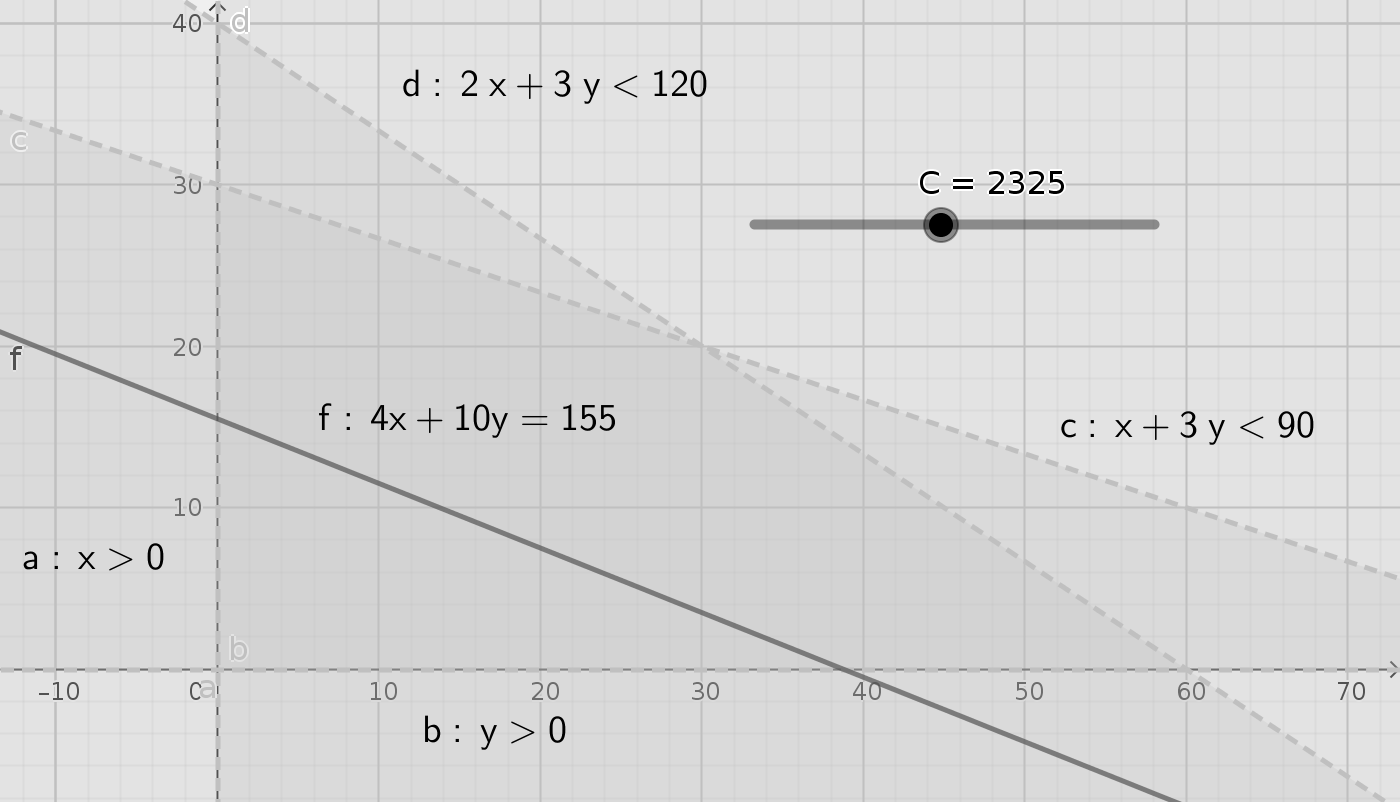
\includegraphics[width=0.8\linewidth]{figs/del2_oppg3}
	\end{center}
	# Vi lager en glider med navn $C$ i Geogebra, og lager deretter linja $60x + 150 y = C$. Dette er den totale fortjenesten, som vi ønsker å maksimere. Ved å endre på $C$ ser vi at maksimal fortjeneste skjer i $(x, y) = (30, 20)$. De bør produsere \answer{30 kasser av type A, og 20 kasser av type B} for maksimal fortjeneste.
	# Dersom Frode kan jobbe 3 timer ekstra erstatter vi ulikheten som begrenser Frodes arbeidstid. Vi legger på 3 timer ekstra:
	\begin{equation*}
		10x + 30y \leq 60 \cdot 15 \quad \rightarrow \quad10x + 30y \leq 60 \cdot (15 + 3)
	\end{equation*}
	Deretter løser vi det nye systemet på samme måte som i forrige deloppgave. Ved å endre på $C$ ser vi at maksimal fortjeneste skjer i $(x, y) = (12, 32)$. De bør produsere \answer{12 kasser av type A, og 32 kasser av type B} for maksimal fortjeneste. Dette er vist på figuren nedenfor.
	
	\begin{center}
		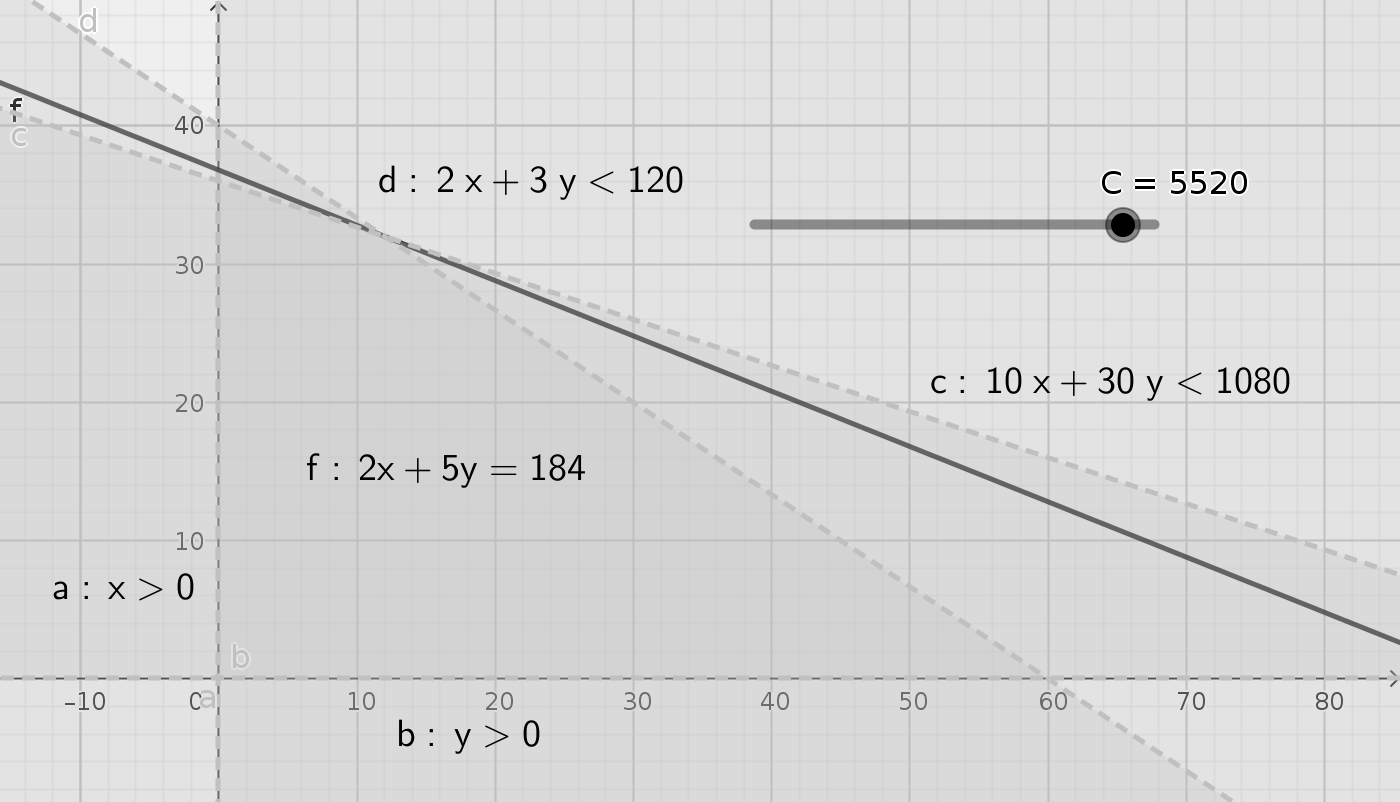
\includegraphics[width=0.8\linewidth]{figs/del2_oppg3_d}
	\end{center}
\end{easylist}

\subsection*{Oppgave 4}
\begin{easylist}[enumerate]
	\ListProperties(Style2*=,Numbers=a,Numbers1=l,FinalMark={)})
	# Vi legger observasjonene inn i regnearket i Geogebra, markerer cellene og velger ``Regresjonsanalyse.'' Tredjegradspolynomet vi får er vist i figuren nedenfor.
	\begin{center}
		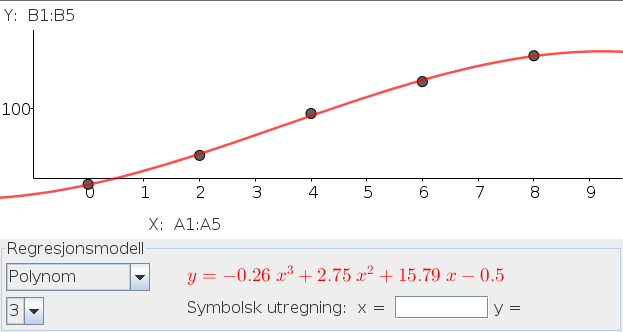
\includegraphics[width=0.8\linewidth]{figs/del2_oppg4a}
	\end{center}
	# Vi bruker \verb|Funksjon(<Funksjon>, <Start>, <Slutt>)|--kommandoen
	for å begrensen funksjonen til $0 \leq x \leq 9$, setter navn på funksjonen i grafikkfeltet og gir navn til aksene.
	\begin{center}
		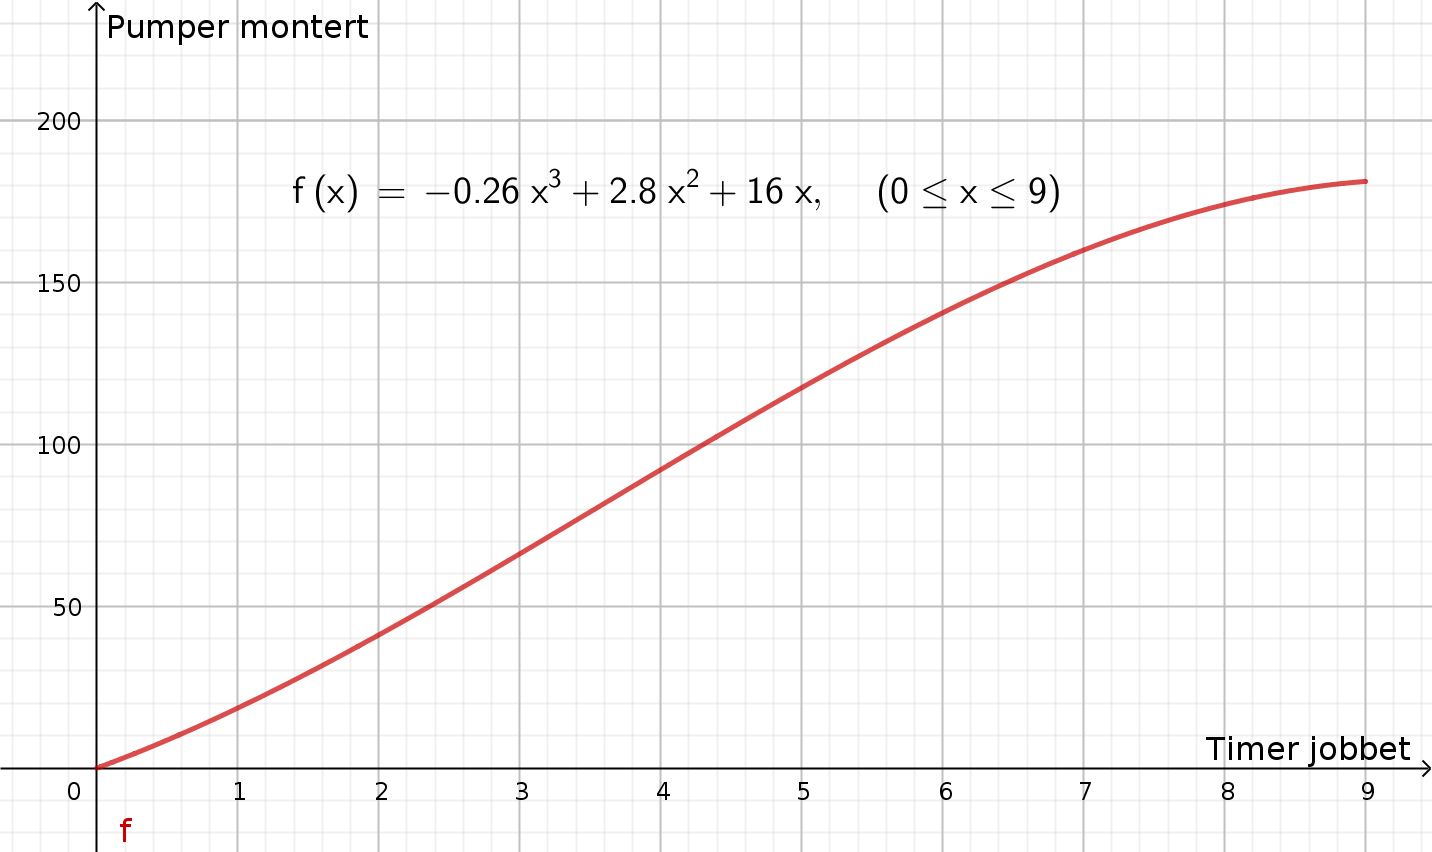
\includegraphics[width=0.8\linewidth]{figs/del2_oppg4b}
	\end{center}
	# La $L_1$ være total lønn når Arne får lønn per pumpe. Den totale lønnen blir
	\begin{equation*}
		L_1(x) = \text{antall pumper} \times \frac{\text{lønn}}{\text{pumpe}}
		= f(x) \times 9.
	\end{equation*}
	La så $L_2$ være total lønn når han får lønn per time. Den totalt lønnen blir da 
	\begin{equation*}
	L_2(x) = \text{antall timer} \times \frac{\text{lønn}}{\text{time}}
	= x \times 190.
	\end{equation*}
	Nedenfor er $L_1(x)$ og $L_2(x)$ plottet i Geogebra. Det lønner seg å velge betaling per monterte pumpe når $L_1(x) > L_2(x)$.
	Vi kan enten finne krysningspunkter, eller finne nullpunktene til differansen $d(x) = L_1(x) - L_2(x)$.
	\begin{center}
		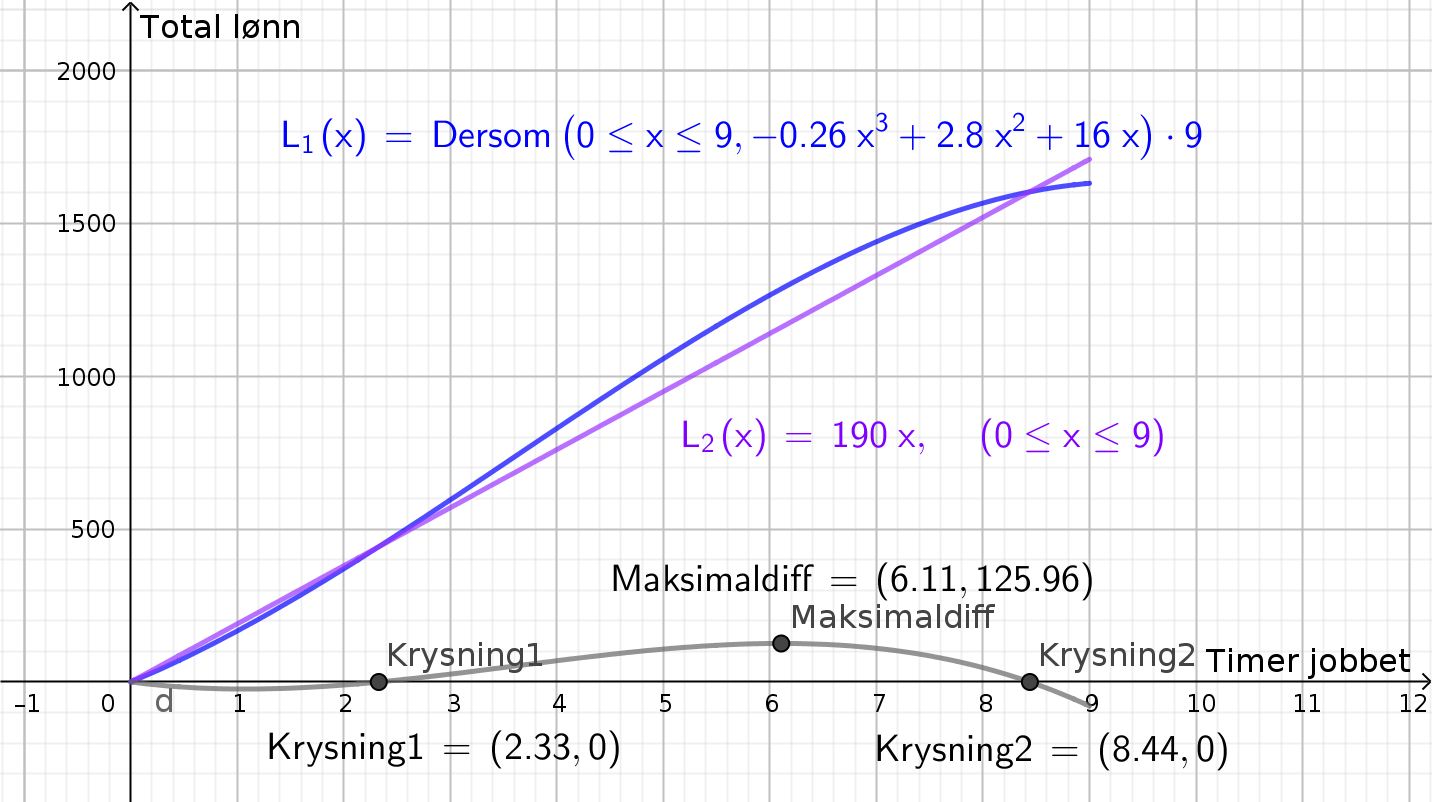
\includegraphics[width=0.8\linewidth]{figs/del2_oppg4_cd}
	\end{center}
	Dersom han jobber hele timer må han jobbe \answer{mellom 3 og 8 timer}.
	Mer presist må han jobbe mellom
	\begin{align*}
		2.33 \text{ timer} = 2 \text{ timer} +  60 \cdot 0.33 \text{ min} &= \text{2 timer og 20 min} \\
		8.44 \text{ timer} = 8 \text{ timer} +  60 \cdot 0.44 \text{ min} &= \text{8 timer og 26 min}
	\end{align*}
	# Vi bruker \verb|Ekstremalpunkt|--kommandoen på differansen $d(x)$. Dette punktet er vist som  ``Maksimaldiff'' ovenfor. Den største forskjellen oppstår etter
	\begin{equation*}
		6.11 \text{ timer} = 6 \text{ timer} +  60 \cdot 0.11 \text{ min} = \answer{\text{6 timer og 7 min}}.
	\end{equation*}
\end{easylist}

\end{document}


